
\section{Лекция 7.}
\subsection{Интегральное уравнение}
% я не ебу как делаются эти новые странички в новых файликах, короче пофиксишь
\deff{def:}  Пусть $f: G \subset \mathbb{R}^{n+1} \to \mathbb{R}^n$. Функция $\varphi: E \to \mathbb{R}^n$ - решение на $E$ интегрального уравнения
$$r(t) = r^0 + \int_{t_0}^{t} f(\tau, r(\tau))\,d\tau,$$
если $E = \langle a, b \rangle$ и $\varphi(t) \equiv r^0 + \int_{t_0}^{t} f(\tau, \varphi(\tau))\,d\tau$ на $E$, где интеграл понимается в смысле Римана. 


\thmm{Лемма (о равносильном интегральном уравнении).}  

Пусть $E = \langle a, b \rangle$, $t_0 \in E$, $G$ - область в $\mathbb{R}^{n+1}$, $(t_0, r^0) \in G$, $f \in C(G \to \mathbb{R}^n)$. Тогда $\varphi$ - решение на $E$ задачи Коши
$$r' = f(t, r), \quad r(t_0) = r^0,$$
если и только если $\varphi$ - решение на $E$ уравнения
$$r(t) = r^0 + \int_{t_0}^{t} f(\tau, r(\tau))\,d\tau.$$
\textbf{Доказательство:}

Пусть $\varphi$ - решение (1) на $E$. Интегрируя равенство $\varphi'(\tau) = f(\tau, \varphi(\tau))$ от $t_0$ до $t \in E$, обе части которого - непрерывные функции, имеем
$$\varphi(t) - \varphi(t_0) = \int_{t_0}^{t} f(\tau, \varphi(\tau))\,d\tau.$$
Поскольку $\varphi(t_0) = r^0$, то функция $\varphi$ - решение уравнения (2) по определению. 

Докажем обратное. Пусть $\varphi$ - решение (2) на $E$.  Тогда из равенства
$$\varphi(t) = r^0 + \int_{t_0}^{t} f(\tau, \varphi(\tau))\,d\tau $$
следует, что $\varphi \in C(E)$.  Отсюда и из (3) вытекает дифференцируемость $\varphi$. Дифференцируя (3) по $t$, получаем: $\varphi'(t) \equiv f(t, \varphi(t))$. Кроме того, из (3) имеем $\varphi(t_0) = r^0$. Таким образом, $\varphi$ - решение задачи (1) по определению. 

\hfill Q.E.D.

\thmm{Лемма (о гладкой стыковке решений).} 

Пусть область $G \subset \mathbb{R}^{n+1}_{t,r}$, $f \in C(G \to \mathbb{R}^n)$, $(t_0, r^0) \in G$, уравнение $r' = f(t, r)$ имеет решения: $\varphi_-$ на $(a, t_0)$, $\varphi_+$ на $(t_0, b)$. Кроме того, $\varphi_-(t_0-) = \varphi_+(t_0+) = r^0$.  Тогда функция
\begin{equation*}\varphi(t) = 
\begin{cases}
\varphi_-(t), & \text{если } t \in (a, t_0), \\
r^0, & \text{если } t = t_0, \\
\varphi_+(t), & \text{если } t \in (t_0, b)
\end{cases}
\end{equation*}
является решением того же уравнения на $(a, b)$.

\textbf{Доказательство:}

Пусть $t, t_- \in (a, t_0)$. По лемме о равносильном интегральном уравнении
$$\varphi_-(t) = \varphi_-(t_-) + \int_{t_-}^{t} f(\tau, \varphi_-(\tau)) \, d\tau.$$

Переходя в этом равенстве к пределу при $t_- \to t_0-$ и замечая, что $\varphi_- = \varphi$ для точек из отрезка $\overline{t, t_-}$, получаем
$$\varphi(t) = r^0 + \int_{t_0}^{t} f(\tau, \varphi(\tau)) \, d\tau.$$

Поступая аналогично для точек $t, t_+ \in (t_0, b)$, при $t_+ \to t_0+$ приходим к равенству (4).

Таким образом, равенство (4) выполнено для всех $t \in (a, b)$. Остается применить лемму о равносильном интегральном уравнении.

\hfill Q.E.D.

\thmm{Лемма (Гронуолл).} 

Пусть $D = \langle a, b \rangle$, $\varphi \in C(D)$, $t_0 \in D$, $\lambda, \mu \geq 0$, при любом $t \in D$ верно двойное неравенство
$$0 \leq \varphi(t) \leq \lambda + \mu \left| \int_{t_0}^{t} \varphi(\tau) \, d\tau \right|.$$
Тогда для любого $t \in D$
$$\varphi(t) \leq \lambda e^{\mu|t - t_0|}.$$

\textbf{Доказательство.} 

Рассмотрим случай $t \geq t_0$ (при $t < t_0$ доказательство аналогично). Положим
$$v(t) = \lambda + \mu \int_{t_0}^{t} \varphi(\tau) \, d\tau.$$

Из данного в условии неравенства имеем $v'(t) = \mu \varphi(t) \leq \mu v(t)$. Умножая полученное неравенство на $e^{-\mu t}$, находим
$$v' e^{-\mu t} - \mu v e^{-\mu t} \leq 0,$$
то есть
$$(v e^{-\mu t})' \leq 0.$$
Следовательно, функция $v e^{-\mu t}$ убывает при $t \geq t_0$. Поэтому
$$v(t) e^{-\mu t} \leq v(t_0) e^{-\mu t_0}.$$
Отсюда
$$\varphi(t) \leq v(t) \leq v(t_0) e^{\mu (t - t_0)} = \lambda e^{\mu (t - t_0)}.$$
\hfill Q.E.D.


\subsection{Теорема существования и единственности}

\deff{def:} Пусть область $G \subset \mathbb{R}_{t,r}^{n+1}$, $(t_0, r^0) \in G$,
$$\Pi := \{(t, r) \in \mathbb{R}^{n+1} \mid |t - t_0| \leq a, |r - r^0| \leq b\},$$
где числа $a, b > 0$ таковы, что $\Pi \subset G$. 

Положим $M = \max\limits_{{(t,r)} \in \Pi} |f(t, r)|$, $h = \min\{a, \frac{b}{M}\}$ (если $M = 0$, то $h := a$). 

Отрезок $[t_0 - h, t_0 + h]$
называется \textbf{отрезком Пеано}, соответствующим точке $(t_0, r^0)$ (рис. 1).

\begin{center}
    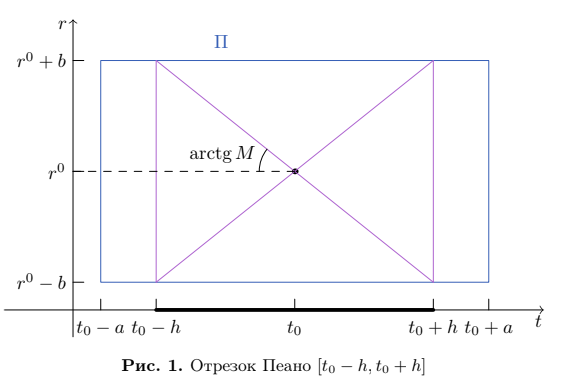
\includegraphics[width=0.7\linewidth]{assets/7-koshi.png}
\end{center}
    


\thmm{Теорема (Пикар, существование и единственность решения ЗК)}

Пусть область $G \subset \mathbb{R}_{t,r}^{n+1}$, $f \in C(G \to \mathbb{R}^n) \cap Lip_{r, loc}$, $(t_0, r^0) \in G$. Тогда
\begin{enumerate}
    \item[(i)] на отрезке Пеано существует решение задачи        
            $$r' = f(t, r), \quad r(t_0) = r^0;$$        
    \item[(ii)] если $\psi_1$ и $\psi_2$ - решения (5), то $\psi_1 \equiv \psi_2$ на $\text{dom } \psi_1 \cap \text{dom } \psi_2$.
\end{enumerate}

\textbf{Доказательство.}

Будем считать, что $t_0 = 0, r^0 = 0$ (в противном случае перенесём начало координат в точку $(t_0, r^0)$). Достаточно установить существование решения на отрезке $[0, h]$ - правой половине отрезка Пеано (рассуждения на $[-h, 0]$ аналогичны, а на всём отрезке решение получается применением леммы о гладкой стыковке).

Пусть
$$\Pi := \{(t, r) \in \mathbb{R}^{n+1} \mid |t| \leq a, |r| \leq b \} \subset G, \quad M := \max_{\Pi} |f|, \quad h = \min \{a, b/M\}.$$

На отрезке $[0, h]$ зададим последовательность функций
$$\varphi_0(t) = 0, $$
$$\varphi_{k+1}(t) = \int_{0}^{t} f(\tau, \varphi_k(\tau)) \, d\tau.$$
Дальнейшую часть доказательства разобьём на этапы:
\begin{enumerate}
    \item Чтобы построить функцию $\varphi_{k+1}$ должно быть $(t, \varphi_{k+1}(t)) \in G$ при всех $t \in [0, h]$. Докажем более сильное утверждение: $(t, \varphi_k(t)) \in \Pi$ при всех $t \in [0, h]$.
    \item Докажем, что последовательность $(\varphi_k)$ равномерно на $[0, h]$ сходится к некоторой функции $\varphi$.
    \item Установим, что $\varphi$ - решение интегрального уравнения, равносильного задаче (5). Тогда останется применить лемму о равносильном интегральном уравнении для завершения доказательства пункта (i).
    \item Докажем единственность (пункт (ii)), применив лемму Гронуолла.
\end{enumerate}

\textbf{1.} При $k=0$, очевидно, $(t, \varphi_k(t)) \in \Pi$. Пусть это верно при некотором $k \in \mathbb{Z}_{+}$. Тогда функция $\varphi_{k+1}$ определена на $[0, h]$ и
$$|\varphi_{k+1}(t)| \leq \int_{0}^{t} |f(\tau, \varphi_k(\tau))| \, d\tau \leq Mt \leq Mh \leq M \frac{b}{M} = b,$$
что влечёт включение $(t, \varphi_{k+1}(t)) \in \Pi$ при всех $t \in [0, h]$.

\textbf{2.} Воспользуемся критерием Коши: установим, что для любого $\varepsilon > 0$ найдётся $N \in \mathbb{N}$, такое что при всех $m \geq N$, всех $k \in \mathbb{N}$ и всех $t \in [0, h]$
$$|\varphi_{m+k}(t) - \varphi_m(t)| \leq \varepsilon.$$
По лемме ?? будет $f \in Lip_r \Pi$ с некоторой константой Липшица $L$. Индукцией по $m$ докажем неравенство
$$|\varphi_{m+k}(t) - \varphi_m(t)| \leq \frac{ML^m t^{m+1}}{(m+1)!}.$$
При $m=0$ утверждение верно, так как
$$|\varphi_k(t) - \varphi_0(t)| \leq \int_{0}^{t} |f(\tau, \varphi_{k-1}(\tau))| \, d\tau \leq Mt.$$
Допуская его справедливость при некотором $m$, имеем
$$|\varphi_{m+1+k}(t) - \varphi_{m+1}(t)| \leq \int_{0}^{t} |f(\tau, \varphi_{m+k}(\tau)) - f(\tau, \varphi_m(\tau))| \, d\tau$$
$$\leq \int_{0}^{t} L |\varphi_{m+k}(\tau) - \varphi_m(\tau)| \, d\tau 
\leq \int_{0}^{t} L \frac{ML^m \tau^{m+1}}{(m+1)!} \, d\tau = \frac{ML^{m+1}t^{m+2}}{(m+2)!}.$$
что и требовалось. Из (6) вытекает, что при любом $t \in [0, h]$
$$|\varphi_{m+k}(t) - \varphi_m(t)| \leq \frac{ML^m h^{m+1}}{(m+1)!}.$$
Выражение в правой части не зависит от $t$ и $k$ и стремится к нулю при $m \to \infty$, поскольку является общим членом ряда Тейлора для экспоненты. Значит, последовательность $(\varphi_m)$ удовлетворяет критерию Коши. Обозначим через $\varphi$ её предел на $[0, h]$.

\textbf{3.} Переходя к пределу при $m \to \infty$ в равенстве
$$\varphi_{m+1}(t) = \int_{0}^{t} f(\tau, \varphi_m(\tau)) \, d\tau,$$
получаем
$$\varphi(t) = \lim_{m \to \infty} \int_{0}^{t} f(\tau, \varphi_m(\tau)) \, d\tau.$$
В пункте 1 было установлено, что $(t, \varphi_m(t)) \in \Pi$ при всех $t \in [0, h]$. Тогда при $m \to \infty$ будет $(t, \varphi(t)) \in \Pi$ при всех таких $t$. Следовательно,
$$|f(\tau, \varphi_m(\tau)) - f(\tau, \varphi(\tau))| \leq L |\varphi_m(\tau) - \varphi(\tau)|.$$
Учитывая равномерную сходимость $\varphi_m$, из данного неравенства следует, что $f(t, \varphi_m(t)) \to f(t, \varphi(t))$ при $m \to \infty$ равномерно на $[0, h]$. Это позволяет внести знак предела под интеграл в (8). После этого по лемме о равносильном интегральном уравнении заключаем, что $\varphi$ - решение задачи (5) на $[0, h]$.

\textbf{4.} Пусть $\psi_1$ и $\psi_2$ - решения (5), $E = \text{dom } \psi_1 \cap \text{dom } \psi_2$. По лемме о равносильном интегральном уравнении
$$\psi_k(t) = \int_{0}^{t} f(\tau, \psi_k(\tau)) \, d\tau, \quad t \in E, \quad k \in \{1, 2\},$$
поэтому
$$|\psi_1(t) - \psi_2(t)| \leq \int_{0}^{t} |f(\tau, \psi_1(\tau)) - f(\tau, \psi_2(\tau))| \, d\tau.$$
Рассмотрим произвольный отрезок $[\alpha, \beta] \subset E$, содержащий ноль. Графики функций $\psi_1$ и $\psi_2$ на $[\alpha, \beta]$ - компактные множества. По лемме ?? найдется постоянная $\tilde{L}$, такая что
$$|f(\tau, \psi_1(\tau)) - f(\tau, \psi_2(\tau))| \leq \tilde{L} |\psi_1(\tau) - \psi_2(\tau)|$$
при всех $\tau \in [\alpha, \beta]$. Следовательно,
$$|\psi_1(t) - \psi_2(t)| \leq \tilde{L} \int_{0}^{t} |\psi_1(\tau) - \psi_2(\tau)| \, d\tau.$$
По лемме Гронуолла будет $|\psi_1(t) - \psi_2(t)| = 0$ на $[\alpha, \beta]$, то есть $\psi_1$ и $\psi_2$ совпадают на $[\alpha, \beta]$. Поскольку отрезок $[\alpha, \beta]$ выбирался произвольно из $E$, то функции $\psi_1$ и $\psi_2$ совпадают и на всём промежутке $E$.

\hfill Q.E.D.

\deff{def:} При доказательстве использовались последовательные приближения Пикара
$$\varphi_0(t) = r^0, \, \,
\varphi_{k+1}(t) = r^0 + \int_{t_0}^{t} f(\tau, \varphi_k(\tau)) \, d\tau.$$
Сформулируем как следствие теорему существования и единственности, условие которой сильнее, но в то же время проще, чем в теореме Пикара

\textbf{Следствие} 

Пусть область $G \subset \mathbb{R}_{t,r}^{n+1}$, $f \in C(G \to \mathbb{R}^n)$, $f'_r \in \text{Mat}_n(C(G))$, $(t_0, r^0) \in G$. Тогда на отрезке Пеано $[t_0 - h, t_0 + h]$ существует решение $\varphi$ задачи Коши.

\textbf{Следствие (теорема существования и единственности для уравнения высшего порядка).} 

Пусть область $G \subset \mathbb{R}_{t,y, y', \dots, y^{(n-1)}}^{n+1}$, $f, f'_y, f'_{y'}, \dots, f'_{y^{(n-1)}} \in C(G)$, $(t_0, y_0, y'_0, \dots, y_0^{(n-1)}) \in G$. Тогда
\begin{enumerate}
    \item[(i)] в некоторой окрестности точки $t_0$ существует решение задачи
    $$
    \begin{cases}
        y^{(n)} = f(t, y, y', \dots, y^{(n-1)}), \\
        y(t_0) = y_0, \quad y'(t_0) = y'_0, \quad \dots, \quad y^{(n-1)}(t_0) = y_0^{(n-1)};
    \end{cases}
    $$
    \item[(ii)] если $\psi_1$ и $\psi_2$ - решения (9), то $\psi_1 \equiv \psi_2$ на $\text{dom } \psi_1 \cap \text{dom } \psi_2$.
\end{enumerate}